%%%%%%%%%%%%%%%%%%%%%%%%%%%%%%%%%%%%%%%%%
% Beamer Presentation
% LaTeX Template
% Version 1.0 (10/11/12)
%
% This template has been downloaded from:
% http://www.LaTeXTemplates.com
%
% License:
% CC BY-NC-SA 3.0 (http://creativecommons.org/licenses/by-nc-sa/3.0/)
%
%%%%%%%%%%%%%%%%%%%%%%%%%%%%%%%%%%%%%%%%%

%----------------------------------------------------------------------------------------
%	PACKAGES AND THEMES
%----------------------------------------------------------------------------------------
\documentclass{beamer}
\usepackage{amsmath, amsthm, amsfonts}
\usepackage{graphicx}
\usepackage{caption}
\usepackage{subcaption}
%%\usepackage[hyperref, UTF8]{ctex}

\mode<presentation> {

% The Beamer class comes with a number of default slide themes
% which change the colors and layouts of slides. Below this is a list
% of all the themes, uncomment each in turn to see what they look like.

%\usetheme{default}
%\usetheme{AnnArbor}
%\usetheme{Antibes}
%\usetheme{Bergen}
%\usetheme{Berkeley}
%\usetheme{Berlin}
%\usetheme{Boadilla}
%\usetheme{CambridgeUS}
%\usetheme{Copenhagen}
%\usetheme{Darmstadt}
%\usetheme{Dresden}
%\usetheme{Frankfurt}
%\usetheme{Goettingen}
%\usetheme{Hannover}
%\usetheme{Ilmenau}
%\usetheme{JuanLesPins}
%\usetheme{Luebeck}
\usetheme{Madrid}
%\usetheme{Malmoe}
%\usetheme{Marburg}
%\usetheme{Montpellier}
%\usetheme{PaloAlto}
%\usetheme{Pittsburgh}
%\usetheme{Rochester}
%\usetheme{Singapore}
%\usetheme{Szeged}
%\usetheme{Warsaw}

% As well as themes, the Beamer class has a number of color themes
% for any slide theme. Uncomment each of these in turn to see how it
% changes the colors of your current slide theme.

%\usecolortheme{albatross}
%\usecolortheme{beaver}
%\usecolortheme{beetle}
%\usecolortheme{crane}
%\usecolortheme{dolphin}
%\usecolortheme{dove}
%\usecolortheme{fly}
%\usecolortheme{lily}
%\usecolortheme{orchid}
%\usecolortheme{rose}
%\usecolortheme{seagull}
%\usecolortheme{seahorse}
%\usecolortheme{whale}
%\usecolortheme{wolverine}

%\setbeamertemplate{footline} % To remove the footer line in all slides uncomment this line
%\setbeamertemplate{footline}[page number] % To replace the footer line in all slides with a simple slide count uncomment this line

%\setbeamertemplate{navigation symbols}{} % To remove the navigation symbols from the bottom of all slides uncomment this line
}

\usepackage{graphicx} % Allows including images
\usepackage{booktabs} % Allows the use of \toprule, \midrule and \bottomrule in tables

%----------------------------------------------------------------------------------------
%	TITLE PAGE
%----------------------------------------------------------------------------------------

\title[Isotopic Approximation]{Isotopic Approximation Implementation Report} % The short title appears at the bottom of every slide, the full title is only on the title page

\author{ZSW} % Your name
\institute[ZJU] % Your institution as it will appear on the bottom of every slide, may be shorthand to save space
{
ZJU\\ % Your institution for the title page
\medskip
%%\textit{john@smith.com} % Your email address
}
\date{\today} % Date, can be changed to a custom date

\begin{document}

\begin{frame}
\titlepage % Print the title page as the first slide
\end{frame}

\begin{frame}
  \begin{block}{Main idea}
    Approximation of complex shapes with simplicial meshes  within error tolerance.
   \end{block}
\end{frame}

\begin{frame} {Implementation Steps}
  \begin{figure}[h]
    \begin{subfigure}[b]{0.23\textwidth}
      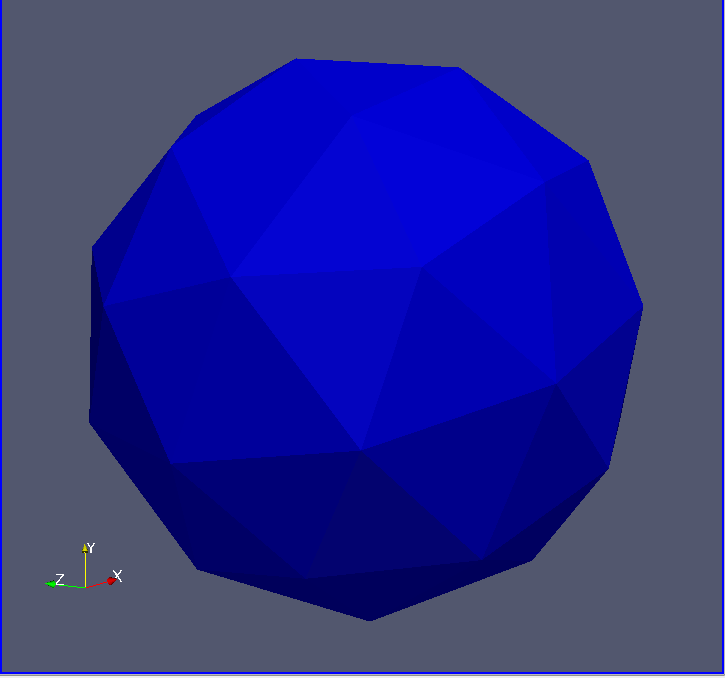
\includegraphics[width=\textwidth]{ori}
      \caption[1]{origional}
    \end{subfigure}
    \begin{subfigure}[b]{0.23\textwidth}
      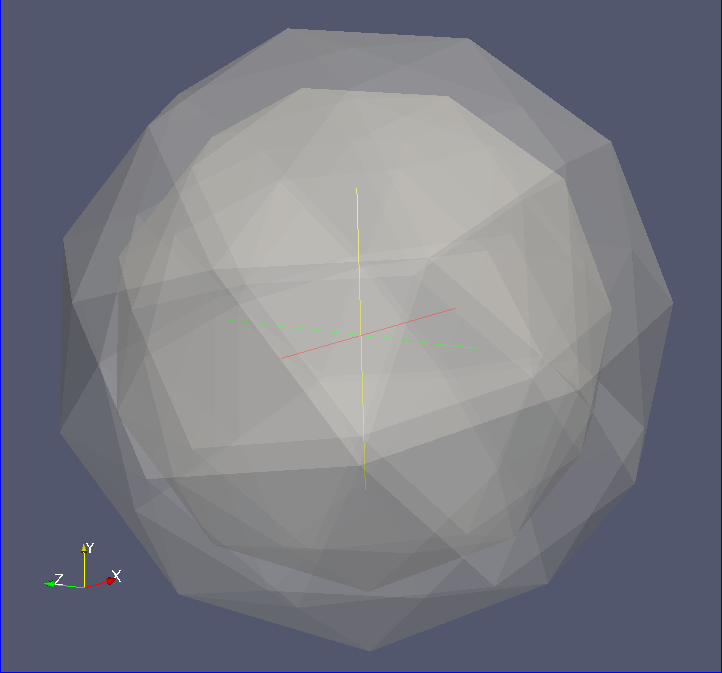
\includegraphics[width=\textwidth]{tol}
      \caption[2]{ tolerance}
    \end{subfigure}
    \begin{subfigure}[b]{0.23\textwidth}
      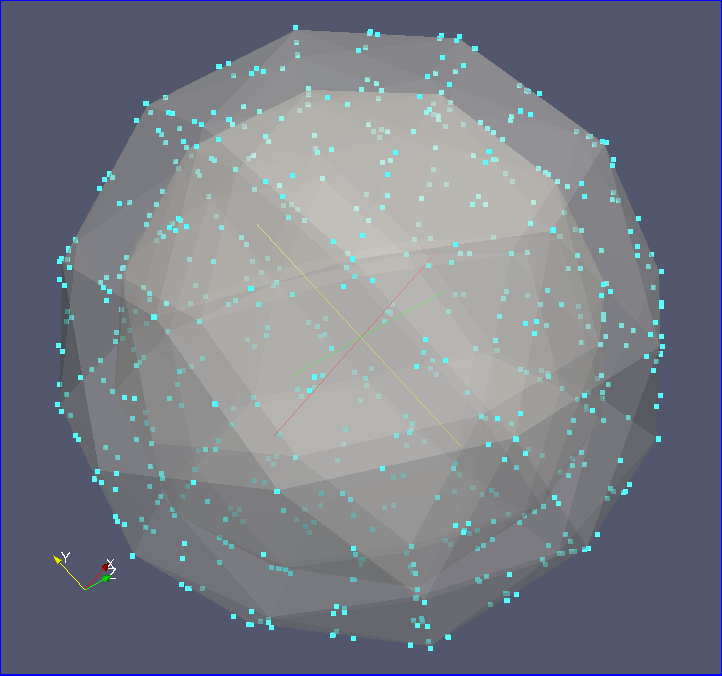
\includegraphics[width=\textwidth]{sampling}
      \caption[3]{sampling}
    \end{subfigure}

    \begin{subfigure}[b]{0.23\textwidth}
      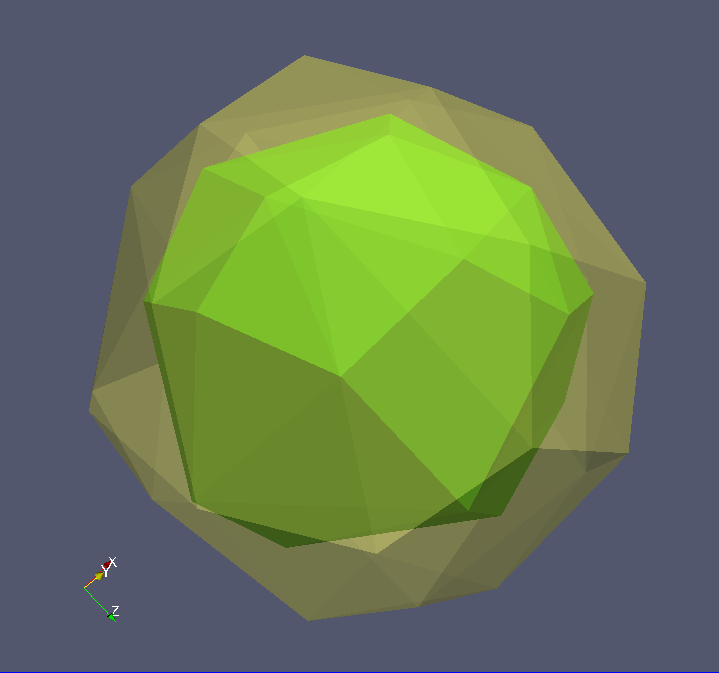
\includegraphics[width=\textwidth]{simp_tol}
      \caption[4]{simp\_tol}
    \end{subfigure}
    \begin{subfigure}[b]{0.23\textwidth}
      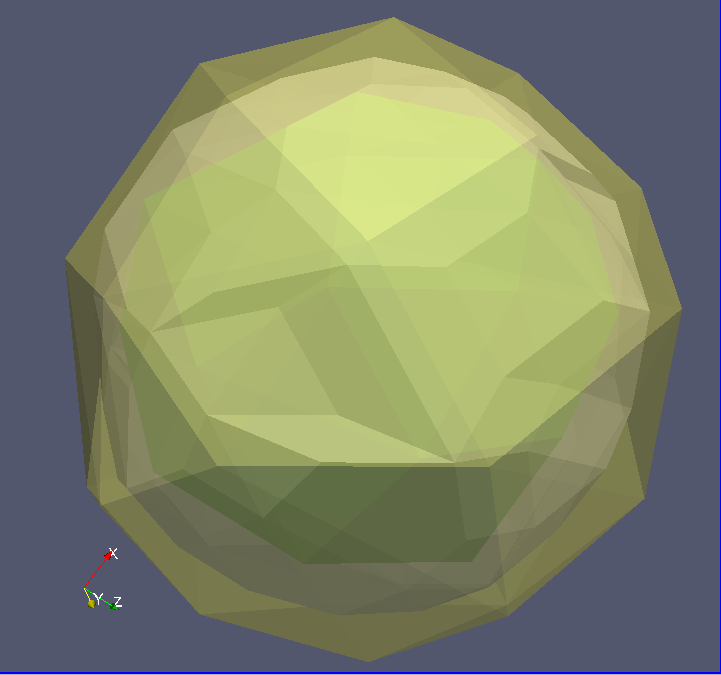
\includegraphics[width=\textwidth]{mutualtesslation}
      \caption[5]{mut-t}
    \end{subfigure}
    \begin{subfigure}[b]{0.23\textwidth}
      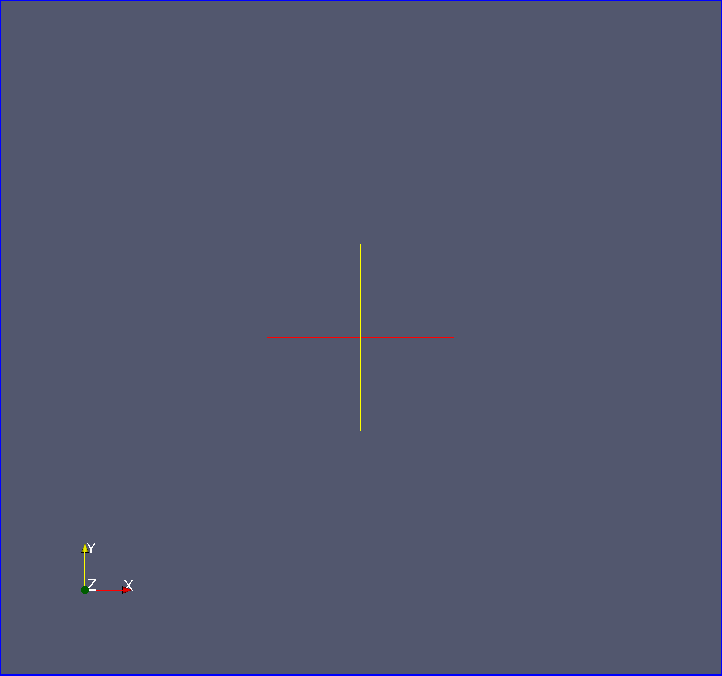
\includegraphics[width=\textwidth]{simp_zero_surface}
      \caption[6]{simp\_z\_surf}
    \end{subfigure}
  \end{figure}
\end{frame}

\begin{frame} {Simplicial Tolerance \& First Condition}
  \begin{figure}[h]
    \begin{subfigure}[b]{0.3\textwidth}
      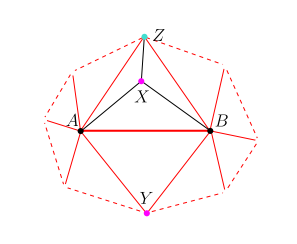
\includegraphics[width=\textwidth]{linkcond1}
      \caption[1]{linkcond1}
    \end{subfigure}
    \begin{subfigure}[b]{0.3\textwidth}
      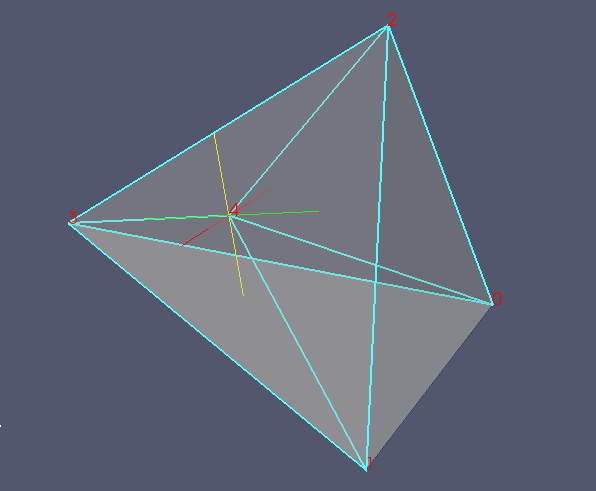
\includegraphics[width=\textwidth]{linkcond2}
      \caption[1]{linkcond2}
    \end{subfigure}
    \caption[linkcond]{\textbf{Link Condition}\\$Lk(A) \cap Lk(B) \ne Lk(AB)$ \&\& no extra edge in Lk(AB)}
  \end{figure}
\end{frame}

\begin{frame} {Simplicial Tolerance \& Second Condition}
  \begin{figure}[h]
    \begin{subfigure}[b]{0.4\textwidth}
      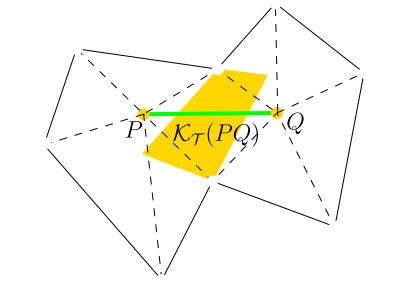
\includegraphics[width=\textwidth]{kr0}
      \caption[kr0]{2D kernel region}
    \end{subfigure}
    \begin{subfigure}[b]{0.4\textwidth}
      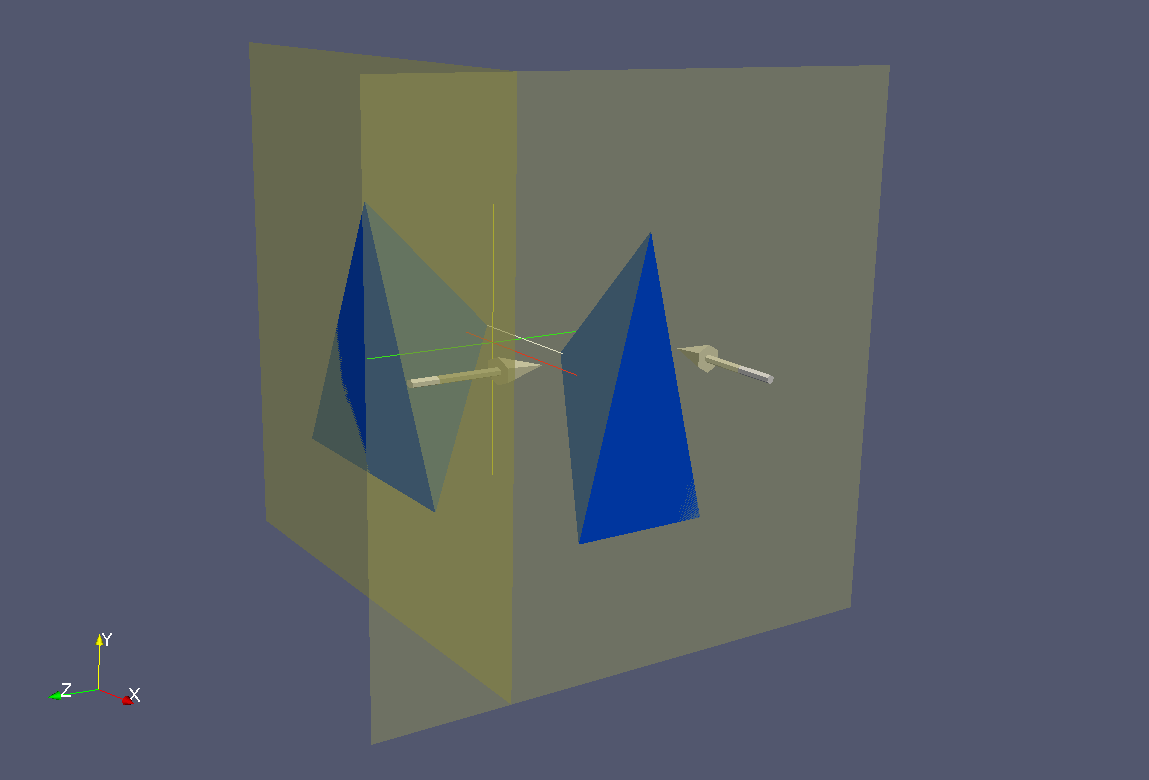
\includegraphics[width=\textwidth]{kr}
      \caption[kr]{3D kernel region}
    \end{subfigure}
    \caption[krcond]{\textbf{Kernel Region Condition}\\ candicate merge point must in kernel region.}
  \end{figure}
\end{frame}

\begin{frame} {Simplicial Tolerance \& Third Condition}
  \begin{figure}[h]
    \begin{subfigure}[b]{0.3\textwidth}
      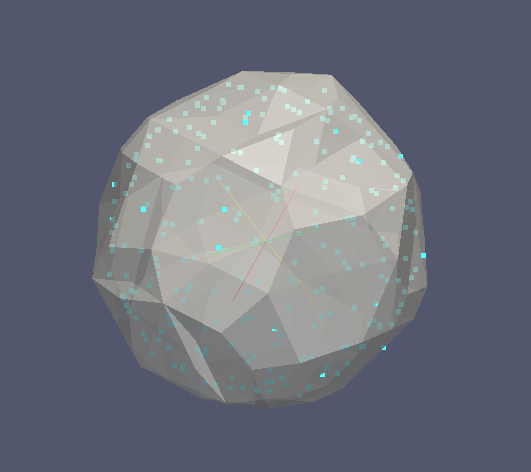
\includegraphics[width=\textwidth]{kp_classification0}
      \caption[kp0]{keep the outer sampling points out of the \textbf{implicit zero surface}}
    \end{subfigure}
    \begin{subfigure}[b]{0.3\textwidth}
      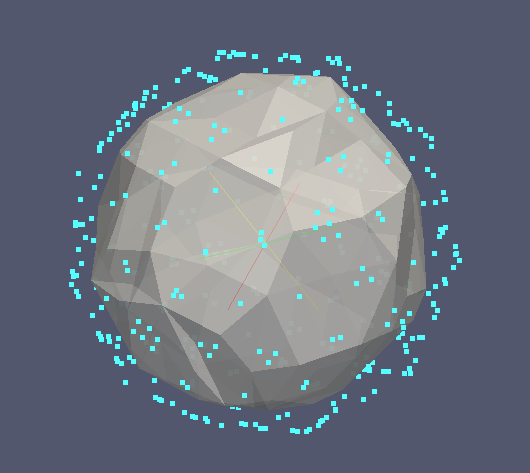
\includegraphics[width=\textwidth]{kp_classification1}
      \caption[kp1]{keep the inner sampling points inner the \textbf{implicit zero surface}}
    \end{subfigure}
    \caption[kp]{\textbf{Keep Classification Condition}\\$fabs(f(s)-F(s))<1$}
  \end{figure}
\end{frame}

\begin{frame} {Implementation Details \& Basic Data Structure}
  \begin{figure}
    \centering
    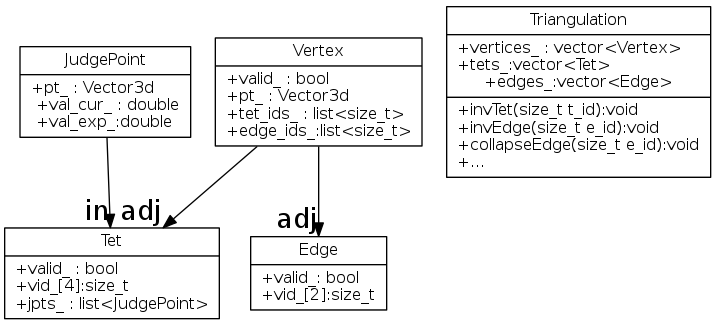
\includegraphics[width=\textwidth] {basic_dt}
    \caption[basic\_dt]{Basic 3d triangulation data structure\\ EdgeCollapse:invalid adj tets and edges, add new tets and edges}
  \end{figure}
\end{frame}

\begin{frame} {Problems \& Precision Problem}
  \begin{figure}
    \begin{subfigure}[b]{0.4\textwidth}
      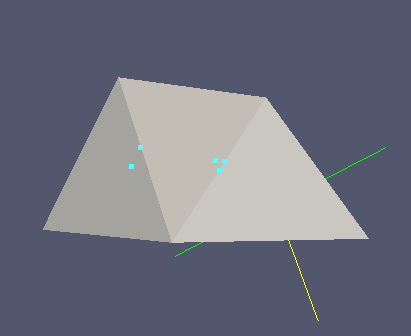
\includegraphics[width=\textwidth]{jbn0}
      \caption[]{Boundary judge problem}
    \end{subfigure}
    \begin{subfigure}[b]{0.4\textwidth}
      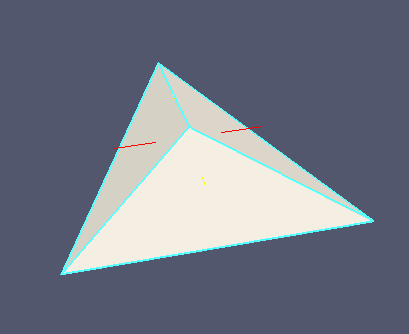
\includegraphics[width=\textwidth]{jbn1}
      \caption[]{Flat tet problem}
    \end{subfigure}
    \caption[]{may lost judge points.}
  \end{figure}
\end{frame}

\begin{frame}%%[plain]
  \begin{columns}
    \begin{column}{\textwidth}
      \begin{center}
        \font\endfont = cmss10 at 25.40mm
        \endfont 
        \baselineskip 20.0mm
        Thank you!
      \end{center}    
    \end{column}
  \end{columns}
\end{frame}
%------------------------------------------------
%----------------------------------------------------------------------------------------

\end{document} 
